\subsection{شبیه‌سازی کانال رول-پیچ استند در حضور کنترل‌کننده LQIDG}\label{roll_pitch_lqidg_section}
در بخش
\ref{quadchanell_roll_pitch}
شبیه‌سازی کانال رول استند چهارپره انجام شد. در این بخش به بررسی عملکرد چهارپره در حضور کنترل‌کننده LQIDG پرداخته می‌شود. کنترل‌کننده LQDG در بخش‌های
\ref{openloop_game}
و
\ref{closedloop_game}
بررسی شده است.
 در شبیه‌سازی برای بهینه‌سازی ضرایب وزنی از روش
TCACS \cite{Karimi2010}
استفاده شده است.
\begin{figure}[H]\label{lqidg_roll_pitch_fig}
	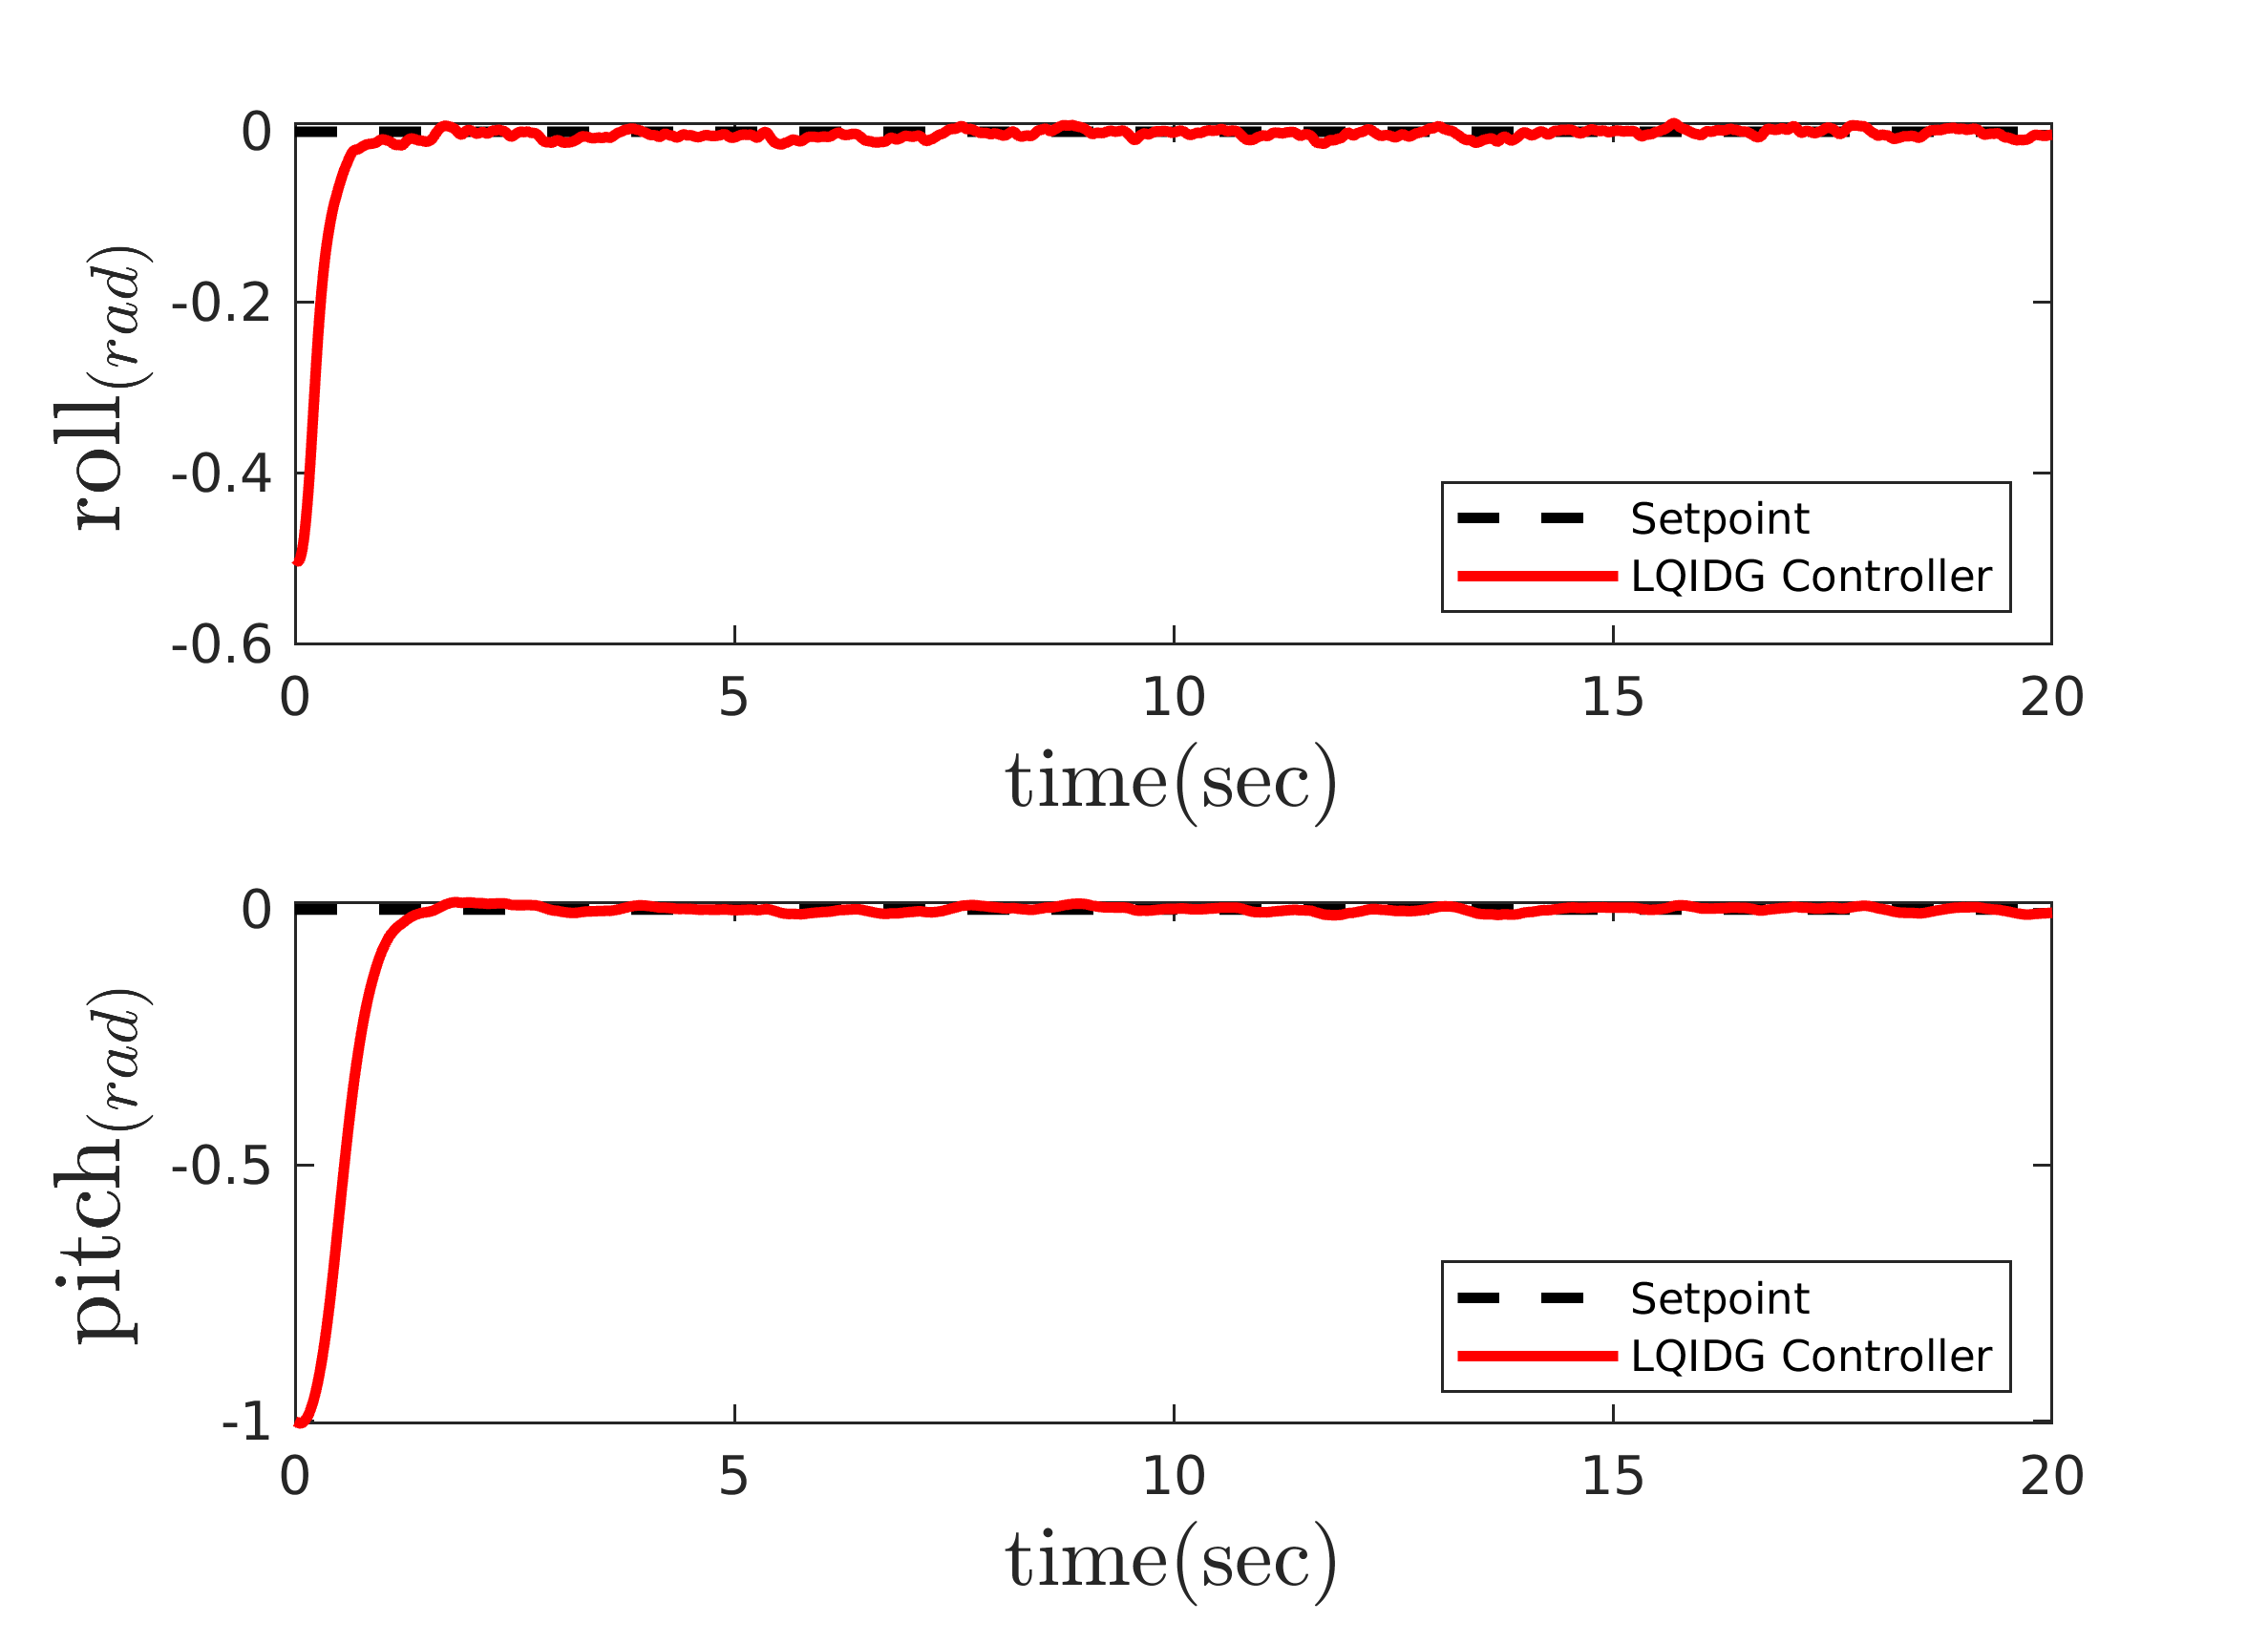
\includegraphics[width=12cm]{../Figures/MIL/LQIDG/Roll_Pitch/lqidg_roll_pitch.png}
	\centering
	\caption{عملكرد LQIDG در کنترل زاويه رول و پیچ (تعقیب ورودی صفر)}
\end{figure}
بر اساس خروجی شبیه‌سازی (شکل
\ref{lqidg_roll_fig})
،کانال رول در حضور کنترل‌کننده LQIDG در حدود پنج ثانیه و کانال پیچ در حدود هشت ثانیه به تعادل می‌رسد و خطای ماندگار آن در حدود صفر است.